\documentclass[twoside]{book}

% Packages required by doxygen
\usepackage{fixltx2e}
\usepackage{calc}
\usepackage{doxygen}
\usepackage[export]{adjustbox} % also loads graphicx
\usepackage{graphicx}
\usepackage[utf8]{inputenc}
\usepackage{makeidx}
\usepackage{multicol}
\usepackage{multirow}
\PassOptionsToPackage{warn}{textcomp}
\usepackage{textcomp}
\usepackage[nointegrals]{wasysym}
\usepackage[table]{xcolor}

% Font selection
\usepackage[T1]{fontenc}
\usepackage[scaled=.90]{helvet}
\usepackage{courier}
\usepackage{amssymb}
\usepackage{sectsty}
\renewcommand{\familydefault}{\sfdefault}
\allsectionsfont{%
  \fontseries{bc}\selectfont%
  \color{darkgray}%
}
\renewcommand{\DoxyLabelFont}{%
  \fontseries{bc}\selectfont%
  \color{darkgray}%
}
\newcommand{\+}{\discretionary{\mbox{\scriptsize$\hookleftarrow$}}{}{}}

% Page & text layout
\usepackage{geometry}
\geometry{%
  a4paper,%
  top=2.5cm,%
  bottom=2.5cm,%
  left=2.5cm,%
  right=2.5cm%
}
\tolerance=750
\hfuzz=15pt
\hbadness=750
\setlength{\emergencystretch}{15pt}
\setlength{\parindent}{0cm}
\setlength{\parskip}{3ex plus 2ex minus 2ex}
\makeatletter
\renewcommand{\paragraph}{%
  \@startsection{paragraph}{4}{0ex}{-1.0ex}{1.0ex}{%
    \normalfont\normalsize\bfseries\SS@parafont%
  }%
}
\renewcommand{\subparagraph}{%
  \@startsection{subparagraph}{5}{0ex}{-1.0ex}{1.0ex}{%
    \normalfont\normalsize\bfseries\SS@subparafont%
  }%
}
\makeatother

% Headers & footers
\usepackage{fancyhdr}
\pagestyle{fancyplain}
\fancyhead[LE]{\fancyplain{}{\bfseries\thepage}}
\fancyhead[CE]{\fancyplain{}{}}
\fancyhead[RE]{\fancyplain{}{\bfseries\leftmark}}
\fancyhead[LO]{\fancyplain{}{\bfseries\rightmark}}
\fancyhead[CO]{\fancyplain{}{}}
\fancyhead[RO]{\fancyplain{}{\bfseries\thepage}}
\fancyfoot[LE]{\fancyplain{}{}}
\fancyfoot[CE]{\fancyplain{}{}}
\fancyfoot[RE]{\fancyplain{}{\bfseries\scriptsize Generated by Doxygen }}
\fancyfoot[LO]{\fancyplain{}{\bfseries\scriptsize Generated by Doxygen }}
\fancyfoot[CO]{\fancyplain{}{}}
\fancyfoot[RO]{\fancyplain{}{}}
\renewcommand{\footrulewidth}{0.4pt}
\renewcommand{\chaptermark}[1]{%
  \markboth{#1}{}%
}
\renewcommand{\sectionmark}[1]{%
  \markright{\thesection\ #1}%
}

% Indices & bibliography
\usepackage{natbib}
\usepackage[titles]{tocloft}
\setcounter{tocdepth}{3}
\setcounter{secnumdepth}{5}
\makeindex

% Hyperlinks (required, but should be loaded last)
\usepackage{ifpdf}
\ifpdf
  \usepackage[pdftex,pagebackref=true]{hyperref}
\else
  \usepackage[ps2pdf,pagebackref=true]{hyperref}
\fi
\hypersetup{%
  colorlinks=true,%
  linkcolor=blue,%
  citecolor=blue,%
  unicode%
}

% Custom commands
\newcommand{\clearemptydoublepage}{%
  \newpage{\pagestyle{empty}\cleardoublepage}%
}

\usepackage{caption}
\captionsetup{labelsep=space,justification=centering,font={bf},singlelinecheck=off,skip=4pt,position=top}

%===== C O N T E N T S =====

\begin{document}

% Titlepage & ToC
\hypersetup{pageanchor=false,
             bookmarksnumbered=true,
             pdfencoding=unicode
            }
\pagenumbering{alph}
\begin{titlepage}
\vspace*{7cm}
\begin{center}%
{\Large L\+D-\/03-\/\+Csharp-\/\+O\+O\+P-\/\+Examples-\/\+U\+ML }\\
\vspace*{1cm}
{\large Generated by Doxygen 1.8.14}\\
\end{center}
\end{titlepage}
\clearemptydoublepage
\pagenumbering{roman}
\tableofcontents
\clearemptydoublepage
\pagenumbering{arabic}
\hypersetup{pageanchor=true}

%--- Begin generated contents ---
\chapter{Namespace Index}
\section{Packages}
Here are the packages with brief descriptions (if available)\+:\begin{DoxyCompactList}
\item\contentsline{section}{\mbox{\hyperlink{namespace_l_d__03___csharp___o_o_p___examples}{L\+D\+\_\+03\+\_\+\+Csharp\+\_\+\+O\+O\+P\+\_\+\+Examples}} }{\pageref{namespace_l_d__03___csharp___o_o_p___examples}}{}
\item\contentsline{section}{\mbox{\hyperlink{namespace_o_o_p_examples}{O\+O\+P\+Examples}} }{\pageref{namespace_o_o_p_examples}}{}
\end{DoxyCompactList}

\chapter{Hierarchical Index}
\section{Class Hierarchy}
This inheritance list is sorted roughly, but not completely, alphabetically\+:\begin{DoxyCompactList}
\item \contentsline{section}{L\+D\+\_\+03\+\_\+\+Csharp\+\_\+\+O\+O\+P\+\_\+\+Examples.\+Computer}{\pageref{class_l_d__03___csharp___o_o_p___examples_1_1_computer}}{}
\begin{DoxyCompactList}
\item \contentsline{section}{L\+D\+\_\+03\+\_\+\+Csharp\+\_\+\+O\+O\+P\+\_\+\+Examples.\+Laptop}{\pageref{class_l_d__03___csharp___o_o_p___examples_1_1_laptop}}{}
\end{DoxyCompactList}
\item \contentsline{section}{O\+O\+P\+Examples.\+Computer}{\pageref{class_o_o_p_examples_1_1_computer}}{}
\item \contentsline{section}{L\+D\+\_\+03\+\_\+\+Csharp\+\_\+\+O\+O\+P\+\_\+\+Examples.\+Display}{\pageref{class_l_d__03___csharp___o_o_p___examples_1_1_display}}{}
\item \contentsline{section}{L\+D\+\_\+03\+\_\+\+Csharp\+\_\+\+O\+O\+P\+\_\+\+Examples.\+I\+Power\+On}{\pageref{interface_l_d__03___csharp___o_o_p___examples_1_1_i_power_on}}{}
\begin{DoxyCompactList}
\item \contentsline{section}{L\+D\+\_\+03\+\_\+\+Csharp\+\_\+\+O\+O\+P\+\_\+\+Examples.\+Power\+Controller}{\pageref{class_l_d__03___csharp___o_o_p___examples_1_1_power_controller}}{}
\end{DoxyCompactList}
\item \contentsline{section}{L\+D\+\_\+03\+\_\+\+Csharp\+\_\+\+O\+O\+P\+\_\+\+Examples.\+I\+Sleep}{\pageref{interface_l_d__03___csharp___o_o_p___examples_1_1_i_sleep}}{}
\begin{DoxyCompactList}
\item \contentsline{section}{L\+D\+\_\+03\+\_\+\+Csharp\+\_\+\+O\+O\+P\+\_\+\+Examples.\+Laptop}{\pageref{class_l_d__03___csharp___o_o_p___examples_1_1_laptop}}{}
\item \contentsline{section}{L\+D\+\_\+03\+\_\+\+Csharp\+\_\+\+O\+O\+P\+\_\+\+Examples.\+Sleep\+Controler}{\pageref{class_l_d__03___csharp___o_o_p___examples_1_1_sleep_controler}}{}
\end{DoxyCompactList}
\item \contentsline{section}{Program}{\pageref{class_program}}{}
\end{DoxyCompactList}

\chapter{Class Index}
\section{Class List}
Here are the classes, structs, unions and interfaces with brief descriptions\+:\begin{DoxyCompactList}
\item\contentsline{section}{\mbox{\hyperlink{class_l_d__03___csharp___o_o_p___examples_1_1_computer}{L\+D\+\_\+03\+\_\+\+Csharp\+\_\+\+O\+O\+P\+\_\+\+Examples.\+Computer}} }{\pageref{class_l_d__03___csharp___o_o_p___examples_1_1_computer}}{}
\item\contentsline{section}{\mbox{\hyperlink{class_o_o_p_examples_1_1_computer}{O\+O\+P\+Examples.\+Computer}} }{\pageref{class_o_o_p_examples_1_1_computer}}{}
\item\contentsline{section}{\mbox{\hyperlink{class_l_d__03___csharp___o_o_p___examples_1_1_display}{L\+D\+\_\+03\+\_\+\+Csharp\+\_\+\+O\+O\+P\+\_\+\+Examples.\+Display}} }{\pageref{class_l_d__03___csharp___o_o_p___examples_1_1_display}}{}
\item\contentsline{section}{\mbox{\hyperlink{interface_l_d__03___csharp___o_o_p___examples_1_1_i_power_on}{L\+D\+\_\+03\+\_\+\+Csharp\+\_\+\+O\+O\+P\+\_\+\+Examples.\+I\+Power\+On}} }{\pageref{interface_l_d__03___csharp___o_o_p___examples_1_1_i_power_on}}{}
\item\contentsline{section}{\mbox{\hyperlink{interface_l_d__03___csharp___o_o_p___examples_1_1_i_sleep}{L\+D\+\_\+03\+\_\+\+Csharp\+\_\+\+O\+O\+P\+\_\+\+Examples.\+I\+Sleep}} }{\pageref{interface_l_d__03___csharp___o_o_p___examples_1_1_i_sleep}}{}
\item\contentsline{section}{\mbox{\hyperlink{class_l_d__03___csharp___o_o_p___examples_1_1_laptop}{L\+D\+\_\+03\+\_\+\+Csharp\+\_\+\+O\+O\+P\+\_\+\+Examples.\+Laptop}} }{\pageref{class_l_d__03___csharp___o_o_p___examples_1_1_laptop}}{}
\item\contentsline{section}{\mbox{\hyperlink{class_l_d__03___csharp___o_o_p___examples_1_1_power_controller}{L\+D\+\_\+03\+\_\+\+Csharp\+\_\+\+O\+O\+P\+\_\+\+Examples.\+Power\+Controller}} }{\pageref{class_l_d__03___csharp___o_o_p___examples_1_1_power_controller}}{}
\item\contentsline{section}{\mbox{\hyperlink{class_program}{Program}} }{\pageref{class_program}}{}
\item\contentsline{section}{\mbox{\hyperlink{class_l_d__03___csharp___o_o_p___examples_1_1_sleep_controler}{L\+D\+\_\+03\+\_\+\+Csharp\+\_\+\+O\+O\+P\+\_\+\+Examples.\+Sleep\+Controler}} }{\pageref{class_l_d__03___csharp___o_o_p___examples_1_1_sleep_controler}}{}
\end{DoxyCompactList}

\chapter{File Index}
\section{File List}
Here is a list of all files with brief descriptions\+:\begin{DoxyCompactList}
\item\contentsline{section}{C\+:/\+Users/thead/source/repos/\+L\+D-\/03-\/\+Csharp-\/\+O\+O\+P-\/\+Examples/\mbox{\hyperlink{_computer_8cs}{Computer.\+cs}} }{\pageref{_computer_8cs}}{}
\item\contentsline{section}{C\+:/\+Users/thead/source/repos/\+L\+D-\/03-\/\+Csharp-\/\+O\+O\+P-\/\+Examples/\mbox{\hyperlink{_desktop_8cs}{Desktop.\+cs}} }{\pageref{_desktop_8cs}}{}
\item\contentsline{section}{C\+:/\+Users/thead/source/repos/\+L\+D-\/03-\/\+Csharp-\/\+O\+O\+P-\/\+Examples/\mbox{\hyperlink{_display_8cs}{Display.\+cs}} }{\pageref{_display_8cs}}{}
\item\contentsline{section}{C\+:/\+Users/thead/source/repos/\+L\+D-\/03-\/\+Csharp-\/\+O\+O\+P-\/\+Examples/\mbox{\hyperlink{_i_power_on_8cs}{I\+Power\+On.\+cs}} }{\pageref{_i_power_on_8cs}}{}
\item\contentsline{section}{C\+:/\+Users/thead/source/repos/\+L\+D-\/03-\/\+Csharp-\/\+O\+O\+P-\/\+Examples/\mbox{\hyperlink{_i_sleep_8cs}{I\+Sleep.\+cs}} }{\pageref{_i_sleep_8cs}}{}
\item\contentsline{section}{C\+:/\+Users/thead/source/repos/\+L\+D-\/03-\/\+Csharp-\/\+O\+O\+P-\/\+Examples/\mbox{\hyperlink{_laptop_8cs}{Laptop.\+cs}} }{\pageref{_laptop_8cs}}{}
\item\contentsline{section}{C\+:/\+Users/thead/source/repos/\+L\+D-\/03-\/\+Csharp-\/\+O\+O\+P-\/\+Examples/\mbox{\hyperlink{_power_controller_8cs}{Power\+Controller.\+cs}} }{\pageref{_power_controller_8cs}}{}
\item\contentsline{section}{C\+:/\+Users/thead/source/repos/\+L\+D-\/03-\/\+Csharp-\/\+O\+O\+P-\/\+Examples/\mbox{\hyperlink{_program_8cs}{Program.\+cs}} }{\pageref{_program_8cs}}{}
\item\contentsline{section}{C\+:/\+Users/thead/source/repos/\+L\+D-\/03-\/\+Csharp-\/\+O\+O\+P-\/\+Examples/\mbox{\hyperlink{_sleep_controler_8cs}{Sleep\+Controler.\+cs}} }{\pageref{_sleep_controler_8cs}}{}
\end{DoxyCompactList}

\chapter{Namespace Documentation}
\hypertarget{namespace_l_d__03___csharp___o_o_p___examples}{}\section{L\+D\+\_\+03\+\_\+\+Csharp\+\_\+\+O\+O\+P\+\_\+\+Examples Namespace Reference}
\label{namespace_l_d__03___csharp___o_o_p___examples}\index{L\+D\+\_\+03\+\_\+\+Csharp\+\_\+\+O\+O\+P\+\_\+\+Examples@{L\+D\+\_\+03\+\_\+\+Csharp\+\_\+\+O\+O\+P\+\_\+\+Examples}}
\subsection*{Classes}
\begin{DoxyCompactItemize}
\item 
class \mbox{\hyperlink{class_l_d__03___csharp___o_o_p___examples_1_1_computer}{Computer}}
\item 
class \mbox{\hyperlink{class_l_d__03___csharp___o_o_p___examples_1_1_display}{Display}}
\item 
interface \mbox{\hyperlink{interface_l_d__03___csharp___o_o_p___examples_1_1_i_power_on}{I\+Power\+On}}
\item 
interface \mbox{\hyperlink{interface_l_d__03___csharp___o_o_p___examples_1_1_i_sleep}{I\+Sleep}}
\item 
class \mbox{\hyperlink{class_l_d__03___csharp___o_o_p___examples_1_1_laptop}{Laptop}}
\item 
class \mbox{\hyperlink{class_l_d__03___csharp___o_o_p___examples_1_1_power_controller}{Power\+Controller}}
\item 
class \mbox{\hyperlink{class_l_d__03___csharp___o_o_p___examples_1_1_sleep_controler}{Sleep\+Controler}}
\end{DoxyCompactItemize}

\hypertarget{namespace_o_o_p_examples}{}\section{O\+O\+P\+Examples Namespace Reference}
\label{namespace_o_o_p_examples}\index{O\+O\+P\+Examples@{O\+O\+P\+Examples}}
\subsection*{Classes}
\begin{DoxyCompactItemize}
\item 
class \mbox{\hyperlink{class_o_o_p_examples_1_1_computer}{Computer}}
\end{DoxyCompactItemize}

\chapter{Class Documentation}
\hypertarget{class_l_d__03___csharp___o_o_p___examples_1_1_computer}{}\section{L\+D\+\_\+03\+\_\+\+Csharp\+\_\+\+O\+O\+P\+\_\+\+Examples.\+Computer Class Reference}
\label{class_l_d__03___csharp___o_o_p___examples_1_1_computer}\index{L\+D\+\_\+03\+\_\+\+Csharp\+\_\+\+O\+O\+P\+\_\+\+Examples.\+Computer@{L\+D\+\_\+03\+\_\+\+Csharp\+\_\+\+O\+O\+P\+\_\+\+Examples.\+Computer}}
Inheritance diagram for L\+D\+\_\+03\+\_\+\+Csharp\+\_\+\+O\+O\+P\+\_\+\+Examples.\+Computer\+:\begin{figure}[H]
\begin{center}
\leavevmode
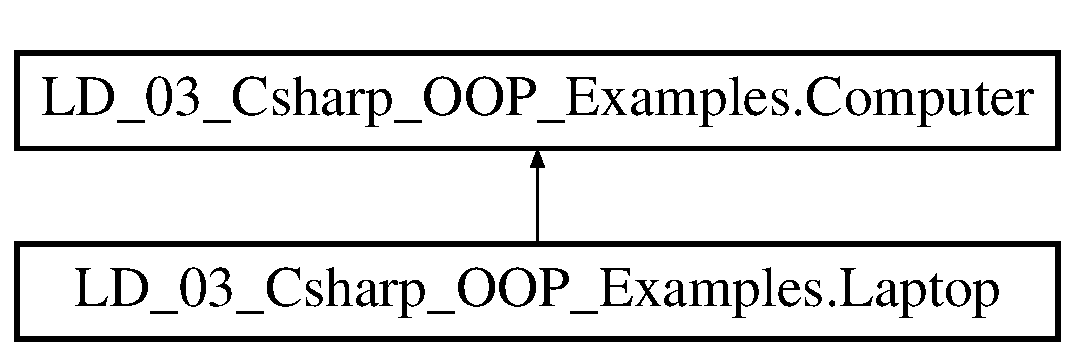
\includegraphics[height=2.000000cm]{class_l_d__03___csharp___o_o_p___examples_1_1_computer}
\end{center}
\end{figure}
\subsection*{Public Member Functions}
\begin{DoxyCompactItemize}
\item 
\mbox{\hyperlink{class_l_d__03___csharp___o_o_p___examples_1_1_computer_a82a05be010b5fa53346c89f89ec91e6d}{Computer}} (string name)
\item 
virtual void \mbox{\hyperlink{class_l_d__03___csharp___o_o_p___examples_1_1_computer_af134a7a02923b27cf3f15a4108354cd5}{Toggle\+Power}} ()
\end{DoxyCompactItemize}
\subsection*{Protected Member Functions}
\begin{DoxyCompactItemize}
\item 
void \mbox{\hyperlink{class_l_d__03___csharp___o_o_p___examples_1_1_computer_a578c225b5842fa789832d8da9731bca0}{Turn\+On}} ()
\item 
void \mbox{\hyperlink{class_l_d__03___csharp___o_o_p___examples_1_1_computer_aa53a1cb176fe267bd05314373b6d114c}{Turn\+Off}} ()
\end{DoxyCompactItemize}
\subsection*{Protected Attributes}
\begin{DoxyCompactItemize}
\item 
string \mbox{\hyperlink{class_l_d__03___csharp___o_o_p___examples_1_1_computer_a98394d23bbf46e8aee551c746d0a0d33}{\+\_\+name}} = \char`\"{}unknown\char`\"{}
\end{DoxyCompactItemize}
\subsection*{Properties}
\begin{DoxyCompactItemize}
\item 
bool \mbox{\hyperlink{class_l_d__03___csharp___o_o_p___examples_1_1_computer_af5570ada25be8618b12a83ea5e712794}{Is\+On}}\hspace{0.3cm}{\ttfamily  \mbox{[}get\mbox{]}}
\item 
virtual string \mbox{\hyperlink{class_l_d__03___csharp___o_o_p___examples_1_1_computer_ac3826d4cda0b12d36f06ed30e3cf8a26}{Name}}\hspace{0.3cm}{\ttfamily  \mbox{[}get\mbox{]}}
\end{DoxyCompactItemize}


\subsection{Constructor \& Destructor Documentation}
\mbox{\Hypertarget{class_l_d__03___csharp___o_o_p___examples_1_1_computer_a82a05be010b5fa53346c89f89ec91e6d}\label{class_l_d__03___csharp___o_o_p___examples_1_1_computer_a82a05be010b5fa53346c89f89ec91e6d}} 
\index{L\+D\+\_\+03\+\_\+\+Csharp\+\_\+\+O\+O\+P\+\_\+\+Examples\+::\+Computer@{L\+D\+\_\+03\+\_\+\+Csharp\+\_\+\+O\+O\+P\+\_\+\+Examples\+::\+Computer}!Computer@{Computer}}
\index{Computer@{Computer}!L\+D\+\_\+03\+\_\+\+Csharp\+\_\+\+O\+O\+P\+\_\+\+Examples\+::\+Computer@{L\+D\+\_\+03\+\_\+\+Csharp\+\_\+\+O\+O\+P\+\_\+\+Examples\+::\+Computer}}
\subsubsection{\texorpdfstring{Computer()}{Computer()}}
{\footnotesize\ttfamily L\+D\+\_\+03\+\_\+\+Csharp\+\_\+\+O\+O\+P\+\_\+\+Examples.\+Computer.\+Computer (\begin{DoxyParamCaption}\item[{string}]{name }\end{DoxyParamCaption})}



\subsection{Member Function Documentation}
\mbox{\Hypertarget{class_l_d__03___csharp___o_o_p___examples_1_1_computer_af134a7a02923b27cf3f15a4108354cd5}\label{class_l_d__03___csharp___o_o_p___examples_1_1_computer_af134a7a02923b27cf3f15a4108354cd5}} 
\index{L\+D\+\_\+03\+\_\+\+Csharp\+\_\+\+O\+O\+P\+\_\+\+Examples\+::\+Computer@{L\+D\+\_\+03\+\_\+\+Csharp\+\_\+\+O\+O\+P\+\_\+\+Examples\+::\+Computer}!Toggle\+Power@{Toggle\+Power}}
\index{Toggle\+Power@{Toggle\+Power}!L\+D\+\_\+03\+\_\+\+Csharp\+\_\+\+O\+O\+P\+\_\+\+Examples\+::\+Computer@{L\+D\+\_\+03\+\_\+\+Csharp\+\_\+\+O\+O\+P\+\_\+\+Examples\+::\+Computer}}
\subsubsection{\texorpdfstring{Toggle\+Power()}{TogglePower()}}
{\footnotesize\ttfamily virtual void L\+D\+\_\+03\+\_\+\+Csharp\+\_\+\+O\+O\+P\+\_\+\+Examples.\+Computer.\+Toggle\+Power (\begin{DoxyParamCaption}{ }\end{DoxyParamCaption})\hspace{0.3cm}{\ttfamily [virtual]}}

\mbox{\Hypertarget{class_l_d__03___csharp___o_o_p___examples_1_1_computer_aa53a1cb176fe267bd05314373b6d114c}\label{class_l_d__03___csharp___o_o_p___examples_1_1_computer_aa53a1cb176fe267bd05314373b6d114c}} 
\index{L\+D\+\_\+03\+\_\+\+Csharp\+\_\+\+O\+O\+P\+\_\+\+Examples\+::\+Computer@{L\+D\+\_\+03\+\_\+\+Csharp\+\_\+\+O\+O\+P\+\_\+\+Examples\+::\+Computer}!Turn\+Off@{Turn\+Off}}
\index{Turn\+Off@{Turn\+Off}!L\+D\+\_\+03\+\_\+\+Csharp\+\_\+\+O\+O\+P\+\_\+\+Examples\+::\+Computer@{L\+D\+\_\+03\+\_\+\+Csharp\+\_\+\+O\+O\+P\+\_\+\+Examples\+::\+Computer}}
\subsubsection{\texorpdfstring{Turn\+Off()}{TurnOff()}}
{\footnotesize\ttfamily void L\+D\+\_\+03\+\_\+\+Csharp\+\_\+\+O\+O\+P\+\_\+\+Examples.\+Computer.\+Turn\+Off (\begin{DoxyParamCaption}{ }\end{DoxyParamCaption})\hspace{0.3cm}{\ttfamily [protected]}}

\mbox{\Hypertarget{class_l_d__03___csharp___o_o_p___examples_1_1_computer_a578c225b5842fa789832d8da9731bca0}\label{class_l_d__03___csharp___o_o_p___examples_1_1_computer_a578c225b5842fa789832d8da9731bca0}} 
\index{L\+D\+\_\+03\+\_\+\+Csharp\+\_\+\+O\+O\+P\+\_\+\+Examples\+::\+Computer@{L\+D\+\_\+03\+\_\+\+Csharp\+\_\+\+O\+O\+P\+\_\+\+Examples\+::\+Computer}!Turn\+On@{Turn\+On}}
\index{Turn\+On@{Turn\+On}!L\+D\+\_\+03\+\_\+\+Csharp\+\_\+\+O\+O\+P\+\_\+\+Examples\+::\+Computer@{L\+D\+\_\+03\+\_\+\+Csharp\+\_\+\+O\+O\+P\+\_\+\+Examples\+::\+Computer}}
\subsubsection{\texorpdfstring{Turn\+On()}{TurnOn()}}
{\footnotesize\ttfamily void L\+D\+\_\+03\+\_\+\+Csharp\+\_\+\+O\+O\+P\+\_\+\+Examples.\+Computer.\+Turn\+On (\begin{DoxyParamCaption}{ }\end{DoxyParamCaption})\hspace{0.3cm}{\ttfamily [protected]}}



\subsection{Member Data Documentation}
\mbox{\Hypertarget{class_l_d__03___csharp___o_o_p___examples_1_1_computer_a98394d23bbf46e8aee551c746d0a0d33}\label{class_l_d__03___csharp___o_o_p___examples_1_1_computer_a98394d23bbf46e8aee551c746d0a0d33}} 
\index{L\+D\+\_\+03\+\_\+\+Csharp\+\_\+\+O\+O\+P\+\_\+\+Examples\+::\+Computer@{L\+D\+\_\+03\+\_\+\+Csharp\+\_\+\+O\+O\+P\+\_\+\+Examples\+::\+Computer}!\+\_\+name@{\+\_\+name}}
\index{\+\_\+name@{\+\_\+name}!L\+D\+\_\+03\+\_\+\+Csharp\+\_\+\+O\+O\+P\+\_\+\+Examples\+::\+Computer@{L\+D\+\_\+03\+\_\+\+Csharp\+\_\+\+O\+O\+P\+\_\+\+Examples\+::\+Computer}}
\subsubsection{\texorpdfstring{\+\_\+name}{\_name}}
{\footnotesize\ttfamily string L\+D\+\_\+03\+\_\+\+Csharp\+\_\+\+O\+O\+P\+\_\+\+Examples.\+Computer.\+\_\+name = \char`\"{}unknown\char`\"{}\hspace{0.3cm}{\ttfamily [protected]}}



\subsection{Property Documentation}
\mbox{\Hypertarget{class_l_d__03___csharp___o_o_p___examples_1_1_computer_af5570ada25be8618b12a83ea5e712794}\label{class_l_d__03___csharp___o_o_p___examples_1_1_computer_af5570ada25be8618b12a83ea5e712794}} 
\index{L\+D\+\_\+03\+\_\+\+Csharp\+\_\+\+O\+O\+P\+\_\+\+Examples\+::\+Computer@{L\+D\+\_\+03\+\_\+\+Csharp\+\_\+\+O\+O\+P\+\_\+\+Examples\+::\+Computer}!Is\+On@{Is\+On}}
\index{Is\+On@{Is\+On}!L\+D\+\_\+03\+\_\+\+Csharp\+\_\+\+O\+O\+P\+\_\+\+Examples\+::\+Computer@{L\+D\+\_\+03\+\_\+\+Csharp\+\_\+\+O\+O\+P\+\_\+\+Examples\+::\+Computer}}
\subsubsection{\texorpdfstring{Is\+On}{IsOn}}
{\footnotesize\ttfamily bool L\+D\+\_\+03\+\_\+\+Csharp\+\_\+\+O\+O\+P\+\_\+\+Examples.\+Computer.\+Is\+On\hspace{0.3cm}{\ttfamily [get]}}

\mbox{\Hypertarget{class_l_d__03___csharp___o_o_p___examples_1_1_computer_ac3826d4cda0b12d36f06ed30e3cf8a26}\label{class_l_d__03___csharp___o_o_p___examples_1_1_computer_ac3826d4cda0b12d36f06ed30e3cf8a26}} 
\index{L\+D\+\_\+03\+\_\+\+Csharp\+\_\+\+O\+O\+P\+\_\+\+Examples\+::\+Computer@{L\+D\+\_\+03\+\_\+\+Csharp\+\_\+\+O\+O\+P\+\_\+\+Examples\+::\+Computer}!Name@{Name}}
\index{Name@{Name}!L\+D\+\_\+03\+\_\+\+Csharp\+\_\+\+O\+O\+P\+\_\+\+Examples\+::\+Computer@{L\+D\+\_\+03\+\_\+\+Csharp\+\_\+\+O\+O\+P\+\_\+\+Examples\+::\+Computer}}
\subsubsection{\texorpdfstring{Name}{Name}}
{\footnotesize\ttfamily virtual string L\+D\+\_\+03\+\_\+\+Csharp\+\_\+\+O\+O\+P\+\_\+\+Examples.\+Computer.\+Name\hspace{0.3cm}{\ttfamily [get]}}



The documentation for this class was generated from the following file\+:\begin{DoxyCompactItemize}
\item 
C\+:/\+Users/thead/source/repos/\+L\+D-\/03-\/\+Csharp-\/\+O\+O\+P-\/\+Examples/\mbox{\hyperlink{_computer_8cs}{Computer.\+cs}}\end{DoxyCompactItemize}

\hypertarget{class_o_o_p_examples_1_1_computer}{}\section{O\+O\+P\+Examples.\+Computer Class Reference}
\label{class_o_o_p_examples_1_1_computer}\index{O\+O\+P\+Examples.\+Computer@{O\+O\+P\+Examples.\+Computer}}
\subsection*{Public Member Functions}
\begin{DoxyCompactItemize}
\item 
\mbox{\hyperlink{class_o_o_p_examples_1_1_computer_ae42250a9cb267a84a1e9c4cb12fca1ac}{Computer}} (string name)
\item 
virtual void \mbox{\hyperlink{class_o_o_p_examples_1_1_computer_ad5fef11d2efb39d91e2e23eeda6c7f68}{Toggle\+Power}} ()
\end{DoxyCompactItemize}
\subsection*{Protected Member Functions}
\begin{DoxyCompactItemize}
\item 
void \mbox{\hyperlink{class_o_o_p_examples_1_1_computer_a9b61ecf3ab167628d80a973abb6d4166}{Turn\+On}} ()
\item 
void \mbox{\hyperlink{class_o_o_p_examples_1_1_computer_acb10f1d4d7156f99c4ed312b49a95a16}{Turn\+Off}} ()
\end{DoxyCompactItemize}
\subsection*{Protected Attributes}
\begin{DoxyCompactItemize}
\item 
string \mbox{\hyperlink{class_o_o_p_examples_1_1_computer_a96460431d655bd0103de79e25011a098}{\+\_\+name}} = \char`\"{}Unknown\char`\"{}
\end{DoxyCompactItemize}
\subsection*{Properties}
\begin{DoxyCompactItemize}
\item 
bool \mbox{\hyperlink{class_o_o_p_examples_1_1_computer_a304cb089cc592030d2d2cd4a856ddb5f}{Is\+On}}\hspace{0.3cm}{\ttfamily  \mbox{[}get\mbox{]}}
\item 
virtual string \mbox{\hyperlink{class_o_o_p_examples_1_1_computer_af43574d61dd28bd460eeeec609f03ae6}{Name}}\hspace{0.3cm}{\ttfamily  \mbox{[}get\mbox{]}}
\end{DoxyCompactItemize}


\subsection{Constructor \& Destructor Documentation}
\mbox{\Hypertarget{class_o_o_p_examples_1_1_computer_ae42250a9cb267a84a1e9c4cb12fca1ac}\label{class_o_o_p_examples_1_1_computer_ae42250a9cb267a84a1e9c4cb12fca1ac}} 
\index{O\+O\+P\+Examples\+::\+Computer@{O\+O\+P\+Examples\+::\+Computer}!Computer@{Computer}}
\index{Computer@{Computer}!O\+O\+P\+Examples\+::\+Computer@{O\+O\+P\+Examples\+::\+Computer}}
\subsubsection{\texorpdfstring{Computer()}{Computer()}}
{\footnotesize\ttfamily O\+O\+P\+Examples.\+Computer.\+Computer (\begin{DoxyParamCaption}\item[{string}]{name }\end{DoxyParamCaption})}



\subsection{Member Function Documentation}
\mbox{\Hypertarget{class_o_o_p_examples_1_1_computer_ad5fef11d2efb39d91e2e23eeda6c7f68}\label{class_o_o_p_examples_1_1_computer_ad5fef11d2efb39d91e2e23eeda6c7f68}} 
\index{O\+O\+P\+Examples\+::\+Computer@{O\+O\+P\+Examples\+::\+Computer}!Toggle\+Power@{Toggle\+Power}}
\index{Toggle\+Power@{Toggle\+Power}!O\+O\+P\+Examples\+::\+Computer@{O\+O\+P\+Examples\+::\+Computer}}
\subsubsection{\texorpdfstring{Toggle\+Power()}{TogglePower()}}
{\footnotesize\ttfamily virtual void O\+O\+P\+Examples.\+Computer.\+Toggle\+Power (\begin{DoxyParamCaption}{ }\end{DoxyParamCaption})\hspace{0.3cm}{\ttfamily [virtual]}}

\mbox{\Hypertarget{class_o_o_p_examples_1_1_computer_acb10f1d4d7156f99c4ed312b49a95a16}\label{class_o_o_p_examples_1_1_computer_acb10f1d4d7156f99c4ed312b49a95a16}} 
\index{O\+O\+P\+Examples\+::\+Computer@{O\+O\+P\+Examples\+::\+Computer}!Turn\+Off@{Turn\+Off}}
\index{Turn\+Off@{Turn\+Off}!O\+O\+P\+Examples\+::\+Computer@{O\+O\+P\+Examples\+::\+Computer}}
\subsubsection{\texorpdfstring{Turn\+Off()}{TurnOff()}}
{\footnotesize\ttfamily void O\+O\+P\+Examples.\+Computer.\+Turn\+Off (\begin{DoxyParamCaption}{ }\end{DoxyParamCaption})\hspace{0.3cm}{\ttfamily [protected]}}

\mbox{\Hypertarget{class_o_o_p_examples_1_1_computer_a9b61ecf3ab167628d80a973abb6d4166}\label{class_o_o_p_examples_1_1_computer_a9b61ecf3ab167628d80a973abb6d4166}} 
\index{O\+O\+P\+Examples\+::\+Computer@{O\+O\+P\+Examples\+::\+Computer}!Turn\+On@{Turn\+On}}
\index{Turn\+On@{Turn\+On}!O\+O\+P\+Examples\+::\+Computer@{O\+O\+P\+Examples\+::\+Computer}}
\subsubsection{\texorpdfstring{Turn\+On()}{TurnOn()}}
{\footnotesize\ttfamily void O\+O\+P\+Examples.\+Computer.\+Turn\+On (\begin{DoxyParamCaption}{ }\end{DoxyParamCaption})\hspace{0.3cm}{\ttfamily [protected]}}



\subsection{Member Data Documentation}
\mbox{\Hypertarget{class_o_o_p_examples_1_1_computer_a96460431d655bd0103de79e25011a098}\label{class_o_o_p_examples_1_1_computer_a96460431d655bd0103de79e25011a098}} 
\index{O\+O\+P\+Examples\+::\+Computer@{O\+O\+P\+Examples\+::\+Computer}!\+\_\+name@{\+\_\+name}}
\index{\+\_\+name@{\+\_\+name}!O\+O\+P\+Examples\+::\+Computer@{O\+O\+P\+Examples\+::\+Computer}}
\subsubsection{\texorpdfstring{\+\_\+name}{\_name}}
{\footnotesize\ttfamily string O\+O\+P\+Examples.\+Computer.\+\_\+name = \char`\"{}Unknown\char`\"{}\hspace{0.3cm}{\ttfamily [protected]}}



\subsection{Property Documentation}
\mbox{\Hypertarget{class_o_o_p_examples_1_1_computer_a304cb089cc592030d2d2cd4a856ddb5f}\label{class_o_o_p_examples_1_1_computer_a304cb089cc592030d2d2cd4a856ddb5f}} 
\index{O\+O\+P\+Examples\+::\+Computer@{O\+O\+P\+Examples\+::\+Computer}!Is\+On@{Is\+On}}
\index{Is\+On@{Is\+On}!O\+O\+P\+Examples\+::\+Computer@{O\+O\+P\+Examples\+::\+Computer}}
\subsubsection{\texorpdfstring{Is\+On}{IsOn}}
{\footnotesize\ttfamily bool O\+O\+P\+Examples.\+Computer.\+Is\+On\hspace{0.3cm}{\ttfamily [get]}}

\mbox{\Hypertarget{class_o_o_p_examples_1_1_computer_af43574d61dd28bd460eeeec609f03ae6}\label{class_o_o_p_examples_1_1_computer_af43574d61dd28bd460eeeec609f03ae6}} 
\index{O\+O\+P\+Examples\+::\+Computer@{O\+O\+P\+Examples\+::\+Computer}!Name@{Name}}
\index{Name@{Name}!O\+O\+P\+Examples\+::\+Computer@{O\+O\+P\+Examples\+::\+Computer}}
\subsubsection{\texorpdfstring{Name}{Name}}
{\footnotesize\ttfamily virtual string O\+O\+P\+Examples.\+Computer.\+Name\hspace{0.3cm}{\ttfamily [get]}}



The documentation for this class was generated from the following file\+:\begin{DoxyCompactItemize}
\item 
C\+:/\+Users/thead/source/repos/\+L\+D-\/03-\/\+Csharp-\/\+O\+O\+P-\/\+Examples/\mbox{\hyperlink{_desktop_8cs}{Desktop.\+cs}}\end{DoxyCompactItemize}

\hypertarget{class_l_d__03___csharp___o_o_p___examples_1_1_display}{}\section{L\+D\+\_\+03\+\_\+\+Csharp\+\_\+\+O\+O\+P\+\_\+\+Examples.\+Display Class Reference}
\label{class_l_d__03___csharp___o_o_p___examples_1_1_display}\index{L\+D\+\_\+03\+\_\+\+Csharp\+\_\+\+O\+O\+P\+\_\+\+Examples.\+Display@{L\+D\+\_\+03\+\_\+\+Csharp\+\_\+\+O\+O\+P\+\_\+\+Examples.\+Display}}
\subsection*{Public Member Functions}
\begin{DoxyCompactItemize}
\item 
\mbox{\hyperlink{class_l_d__03___csharp___o_o_p___examples_1_1_display_a708bc33cb5d69b49479879c2874b2937}{Display}} (int width, int height)
\end{DoxyCompactItemize}
\subsection*{Properties}
\begin{DoxyCompactItemize}
\item 
int \mbox{\hyperlink{class_l_d__03___csharp___o_o_p___examples_1_1_display_a2bf6c49221f4a135cb99ba3af08a7777}{With}}\hspace{0.3cm}{\ttfamily  \mbox{[}get\mbox{]}}
\item 
int \mbox{\hyperlink{class_l_d__03___csharp___o_o_p___examples_1_1_display_a298ac1d104bf6a51706ee92dec43a2f9}{Heigth}}\hspace{0.3cm}{\ttfamily  \mbox{[}get\mbox{]}}
\end{DoxyCompactItemize}


\subsection{Constructor \& Destructor Documentation}
\mbox{\Hypertarget{class_l_d__03___csharp___o_o_p___examples_1_1_display_a708bc33cb5d69b49479879c2874b2937}\label{class_l_d__03___csharp___o_o_p___examples_1_1_display_a708bc33cb5d69b49479879c2874b2937}} 
\index{L\+D\+\_\+03\+\_\+\+Csharp\+\_\+\+O\+O\+P\+\_\+\+Examples\+::\+Display@{L\+D\+\_\+03\+\_\+\+Csharp\+\_\+\+O\+O\+P\+\_\+\+Examples\+::\+Display}!Display@{Display}}
\index{Display@{Display}!L\+D\+\_\+03\+\_\+\+Csharp\+\_\+\+O\+O\+P\+\_\+\+Examples\+::\+Display@{L\+D\+\_\+03\+\_\+\+Csharp\+\_\+\+O\+O\+P\+\_\+\+Examples\+::\+Display}}
\subsubsection{\texorpdfstring{Display()}{Display()}}
{\footnotesize\ttfamily L\+D\+\_\+03\+\_\+\+Csharp\+\_\+\+O\+O\+P\+\_\+\+Examples.\+Display.\+Display (\begin{DoxyParamCaption}\item[{int}]{width,  }\item[{int}]{height }\end{DoxyParamCaption})}



\subsection{Property Documentation}
\mbox{\Hypertarget{class_l_d__03___csharp___o_o_p___examples_1_1_display_a298ac1d104bf6a51706ee92dec43a2f9}\label{class_l_d__03___csharp___o_o_p___examples_1_1_display_a298ac1d104bf6a51706ee92dec43a2f9}} 
\index{L\+D\+\_\+03\+\_\+\+Csharp\+\_\+\+O\+O\+P\+\_\+\+Examples\+::\+Display@{L\+D\+\_\+03\+\_\+\+Csharp\+\_\+\+O\+O\+P\+\_\+\+Examples\+::\+Display}!Heigth@{Heigth}}
\index{Heigth@{Heigth}!L\+D\+\_\+03\+\_\+\+Csharp\+\_\+\+O\+O\+P\+\_\+\+Examples\+::\+Display@{L\+D\+\_\+03\+\_\+\+Csharp\+\_\+\+O\+O\+P\+\_\+\+Examples\+::\+Display}}
\subsubsection{\texorpdfstring{Heigth}{Heigth}}
{\footnotesize\ttfamily int L\+D\+\_\+03\+\_\+\+Csharp\+\_\+\+O\+O\+P\+\_\+\+Examples.\+Display.\+Heigth\hspace{0.3cm}{\ttfamily [get]}}

\mbox{\Hypertarget{class_l_d__03___csharp___o_o_p___examples_1_1_display_a2bf6c49221f4a135cb99ba3af08a7777}\label{class_l_d__03___csharp___o_o_p___examples_1_1_display_a2bf6c49221f4a135cb99ba3af08a7777}} 
\index{L\+D\+\_\+03\+\_\+\+Csharp\+\_\+\+O\+O\+P\+\_\+\+Examples\+::\+Display@{L\+D\+\_\+03\+\_\+\+Csharp\+\_\+\+O\+O\+P\+\_\+\+Examples\+::\+Display}!With@{With}}
\index{With@{With}!L\+D\+\_\+03\+\_\+\+Csharp\+\_\+\+O\+O\+P\+\_\+\+Examples\+::\+Display@{L\+D\+\_\+03\+\_\+\+Csharp\+\_\+\+O\+O\+P\+\_\+\+Examples\+::\+Display}}
\subsubsection{\texorpdfstring{With}{With}}
{\footnotesize\ttfamily int L\+D\+\_\+03\+\_\+\+Csharp\+\_\+\+O\+O\+P\+\_\+\+Examples.\+Display.\+With\hspace{0.3cm}{\ttfamily [get]}}



The documentation for this class was generated from the following file\+:\begin{DoxyCompactItemize}
\item 
C\+:/\+Users/thead/source/repos/\+L\+D-\/03-\/\+Csharp-\/\+O\+O\+P-\/\+Examples/\mbox{\hyperlink{_display_8cs}{Display.\+cs}}\end{DoxyCompactItemize}

\hypertarget{interface_l_d__03___csharp___o_o_p___examples_1_1_i_power_on}{}\section{L\+D\+\_\+03\+\_\+\+Csharp\+\_\+\+O\+O\+P\+\_\+\+Examples.\+I\+Power\+On Interface Reference}
\label{interface_l_d__03___csharp___o_o_p___examples_1_1_i_power_on}\index{L\+D\+\_\+03\+\_\+\+Csharp\+\_\+\+O\+O\+P\+\_\+\+Examples.\+I\+Power\+On@{L\+D\+\_\+03\+\_\+\+Csharp\+\_\+\+O\+O\+P\+\_\+\+Examples.\+I\+Power\+On}}
Inheritance diagram for L\+D\+\_\+03\+\_\+\+Csharp\+\_\+\+O\+O\+P\+\_\+\+Examples.\+I\+Power\+On\+:\begin{figure}[H]
\begin{center}
\leavevmode
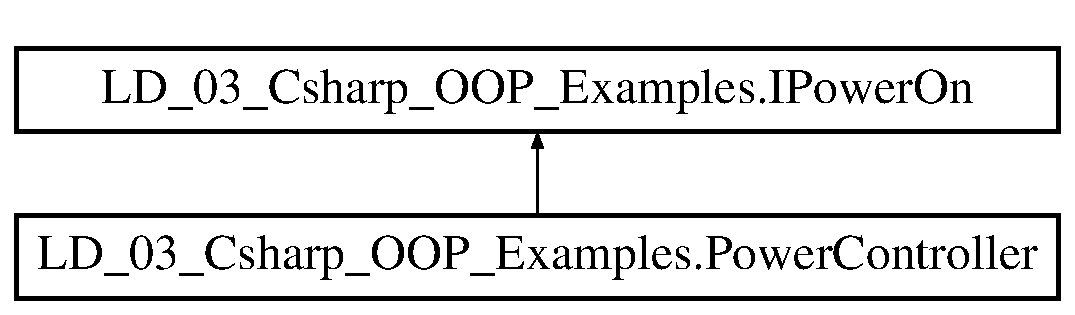
\includegraphics[height=2.000000cm]{interface_l_d__03___csharp___o_o_p___examples_1_1_i_power_on}
\end{center}
\end{figure}
\subsection*{Public Member Functions}
\begin{DoxyCompactItemize}
\item 
void \mbox{\hyperlink{interface_l_d__03___csharp___o_o_p___examples_1_1_i_power_on_a6f71e842b3e94a5d6d690671197d0adc}{Toggle\+Power}} ()
\end{DoxyCompactItemize}
\subsection*{Properties}
\begin{DoxyCompactItemize}
\item 
bool \mbox{\hyperlink{interface_l_d__03___csharp___o_o_p___examples_1_1_i_power_on_ac1162237fd45586cb8f98e42a4778402}{Is\+On}}\hspace{0.3cm}{\ttfamily  \mbox{[}get\mbox{]}}
\end{DoxyCompactItemize}


\subsection{Member Function Documentation}
\mbox{\Hypertarget{interface_l_d__03___csharp___o_o_p___examples_1_1_i_power_on_a6f71e842b3e94a5d6d690671197d0adc}\label{interface_l_d__03___csharp___o_o_p___examples_1_1_i_power_on_a6f71e842b3e94a5d6d690671197d0adc}} 
\index{L\+D\+\_\+03\+\_\+\+Csharp\+\_\+\+O\+O\+P\+\_\+\+Examples\+::\+I\+Power\+On@{L\+D\+\_\+03\+\_\+\+Csharp\+\_\+\+O\+O\+P\+\_\+\+Examples\+::\+I\+Power\+On}!Toggle\+Power@{Toggle\+Power}}
\index{Toggle\+Power@{Toggle\+Power}!L\+D\+\_\+03\+\_\+\+Csharp\+\_\+\+O\+O\+P\+\_\+\+Examples\+::\+I\+Power\+On@{L\+D\+\_\+03\+\_\+\+Csharp\+\_\+\+O\+O\+P\+\_\+\+Examples\+::\+I\+Power\+On}}
\subsubsection{\texorpdfstring{Toggle\+Power()}{TogglePower()}}
{\footnotesize\ttfamily void L\+D\+\_\+03\+\_\+\+Csharp\+\_\+\+O\+O\+P\+\_\+\+Examples.\+I\+Power\+On.\+Toggle\+Power (\begin{DoxyParamCaption}{ }\end{DoxyParamCaption})}



Implemented in \mbox{\hyperlink{class_l_d__03___csharp___o_o_p___examples_1_1_power_controller_accb660a5257db2d4d1df4e35d4147027}{L\+D\+\_\+03\+\_\+\+Csharp\+\_\+\+O\+O\+P\+\_\+\+Examples.\+Power\+Controller}}.



\subsection{Property Documentation}
\mbox{\Hypertarget{interface_l_d__03___csharp___o_o_p___examples_1_1_i_power_on_ac1162237fd45586cb8f98e42a4778402}\label{interface_l_d__03___csharp___o_o_p___examples_1_1_i_power_on_ac1162237fd45586cb8f98e42a4778402}} 
\index{L\+D\+\_\+03\+\_\+\+Csharp\+\_\+\+O\+O\+P\+\_\+\+Examples\+::\+I\+Power\+On@{L\+D\+\_\+03\+\_\+\+Csharp\+\_\+\+O\+O\+P\+\_\+\+Examples\+::\+I\+Power\+On}!Is\+On@{Is\+On}}
\index{Is\+On@{Is\+On}!L\+D\+\_\+03\+\_\+\+Csharp\+\_\+\+O\+O\+P\+\_\+\+Examples\+::\+I\+Power\+On@{L\+D\+\_\+03\+\_\+\+Csharp\+\_\+\+O\+O\+P\+\_\+\+Examples\+::\+I\+Power\+On}}
\subsubsection{\texorpdfstring{Is\+On}{IsOn}}
{\footnotesize\ttfamily bool L\+D\+\_\+03\+\_\+\+Csharp\+\_\+\+O\+O\+P\+\_\+\+Examples.\+I\+Power\+On.\+Is\+On\hspace{0.3cm}{\ttfamily [get]}}



The documentation for this interface was generated from the following file\+:\begin{DoxyCompactItemize}
\item 
C\+:/\+Users/thead/source/repos/\+L\+D-\/03-\/\+Csharp-\/\+O\+O\+P-\/\+Examples/\mbox{\hyperlink{_i_power_on_8cs}{I\+Power\+On.\+cs}}\end{DoxyCompactItemize}

\hypertarget{interface_l_d__03___csharp___o_o_p___examples_1_1_i_sleep}{}\section{L\+D\+\_\+03\+\_\+\+Csharp\+\_\+\+O\+O\+P\+\_\+\+Examples.\+I\+Sleep Interface Reference}
\label{interface_l_d__03___csharp___o_o_p___examples_1_1_i_sleep}\index{L\+D\+\_\+03\+\_\+\+Csharp\+\_\+\+O\+O\+P\+\_\+\+Examples.\+I\+Sleep@{L\+D\+\_\+03\+\_\+\+Csharp\+\_\+\+O\+O\+P\+\_\+\+Examples.\+I\+Sleep}}
Inheritance diagram for L\+D\+\_\+03\+\_\+\+Csharp\+\_\+\+O\+O\+P\+\_\+\+Examples.\+I\+Sleep\+:\begin{figure}[H]
\begin{center}
\leavevmode
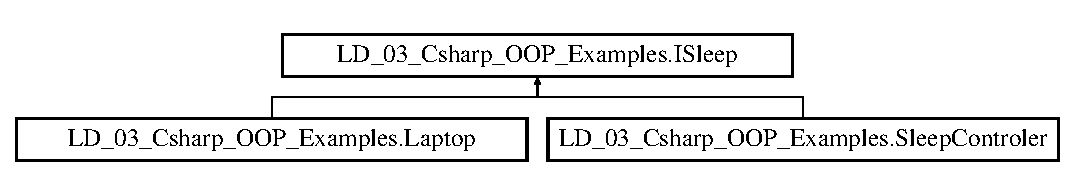
\includegraphics[height=1.937716cm]{interface_l_d__03___csharp___o_o_p___examples_1_1_i_sleep}
\end{center}
\end{figure}
\subsection*{Public Member Functions}
\begin{DoxyCompactItemize}
\item 
void \mbox{\hyperlink{interface_l_d__03___csharp___o_o_p___examples_1_1_i_sleep_a51a16beac9cf61fd4d088e169790bd08}{Toggle\+Sleep}} ()
\end{DoxyCompactItemize}
\subsection*{Properties}
\begin{DoxyCompactItemize}
\item 
bool \mbox{\hyperlink{interface_l_d__03___csharp___o_o_p___examples_1_1_i_sleep_a676dbf702e3243c35818e41970b77d90}{Is\+Sleeping}}\hspace{0.3cm}{\ttfamily  \mbox{[}get\mbox{]}}
\end{DoxyCompactItemize}


\subsection{Member Function Documentation}
\mbox{\Hypertarget{interface_l_d__03___csharp___o_o_p___examples_1_1_i_sleep_a51a16beac9cf61fd4d088e169790bd08}\label{interface_l_d__03___csharp___o_o_p___examples_1_1_i_sleep_a51a16beac9cf61fd4d088e169790bd08}} 
\index{L\+D\+\_\+03\+\_\+\+Csharp\+\_\+\+O\+O\+P\+\_\+\+Examples\+::\+I\+Sleep@{L\+D\+\_\+03\+\_\+\+Csharp\+\_\+\+O\+O\+P\+\_\+\+Examples\+::\+I\+Sleep}!Toggle\+Sleep@{Toggle\+Sleep}}
\index{Toggle\+Sleep@{Toggle\+Sleep}!L\+D\+\_\+03\+\_\+\+Csharp\+\_\+\+O\+O\+P\+\_\+\+Examples\+::\+I\+Sleep@{L\+D\+\_\+03\+\_\+\+Csharp\+\_\+\+O\+O\+P\+\_\+\+Examples\+::\+I\+Sleep}}
\subsubsection{\texorpdfstring{Toggle\+Sleep()}{ToggleSleep()}}
{\footnotesize\ttfamily void L\+D\+\_\+03\+\_\+\+Csharp\+\_\+\+O\+O\+P\+\_\+\+Examples.\+I\+Sleep.\+Toggle\+Sleep (\begin{DoxyParamCaption}{ }\end{DoxyParamCaption})}



Implemented in \mbox{\hyperlink{class_l_d__03___csharp___o_o_p___examples_1_1_laptop_a28f09dd23331929b11cdc77720153e21}{L\+D\+\_\+03\+\_\+\+Csharp\+\_\+\+O\+O\+P\+\_\+\+Examples.\+Laptop}}, and \mbox{\hyperlink{class_l_d__03___csharp___o_o_p___examples_1_1_sleep_controler_ad8b90b3fa29e24828b2d739961458dba}{L\+D\+\_\+03\+\_\+\+Csharp\+\_\+\+O\+O\+P\+\_\+\+Examples.\+Sleep\+Controler}}.



\subsection{Property Documentation}
\mbox{\Hypertarget{interface_l_d__03___csharp___o_o_p___examples_1_1_i_sleep_a676dbf702e3243c35818e41970b77d90}\label{interface_l_d__03___csharp___o_o_p___examples_1_1_i_sleep_a676dbf702e3243c35818e41970b77d90}} 
\index{L\+D\+\_\+03\+\_\+\+Csharp\+\_\+\+O\+O\+P\+\_\+\+Examples\+::\+I\+Sleep@{L\+D\+\_\+03\+\_\+\+Csharp\+\_\+\+O\+O\+P\+\_\+\+Examples\+::\+I\+Sleep}!Is\+Sleeping@{Is\+Sleeping}}
\index{Is\+Sleeping@{Is\+Sleeping}!L\+D\+\_\+03\+\_\+\+Csharp\+\_\+\+O\+O\+P\+\_\+\+Examples\+::\+I\+Sleep@{L\+D\+\_\+03\+\_\+\+Csharp\+\_\+\+O\+O\+P\+\_\+\+Examples\+::\+I\+Sleep}}
\subsubsection{\texorpdfstring{Is\+Sleeping}{IsSleeping}}
{\footnotesize\ttfamily bool L\+D\+\_\+03\+\_\+\+Csharp\+\_\+\+O\+O\+P\+\_\+\+Examples.\+I\+Sleep.\+Is\+Sleeping\hspace{0.3cm}{\ttfamily [get]}}



The documentation for this interface was generated from the following file\+:\begin{DoxyCompactItemize}
\item 
C\+:/\+Users/thead/source/repos/\+L\+D-\/03-\/\+Csharp-\/\+O\+O\+P-\/\+Examples/\mbox{\hyperlink{_i_sleep_8cs}{I\+Sleep.\+cs}}\end{DoxyCompactItemize}

\hypertarget{class_l_d__03___csharp___o_o_p___examples_1_1_laptop}{}\section{L\+D\+\_\+03\+\_\+\+Csharp\+\_\+\+O\+O\+P\+\_\+\+Examples.\+Laptop Class Reference}
\label{class_l_d__03___csharp___o_o_p___examples_1_1_laptop}\index{L\+D\+\_\+03\+\_\+\+Csharp\+\_\+\+O\+O\+P\+\_\+\+Examples.\+Laptop@{L\+D\+\_\+03\+\_\+\+Csharp\+\_\+\+O\+O\+P\+\_\+\+Examples.\+Laptop}}
Inheritance diagram for L\+D\+\_\+03\+\_\+\+Csharp\+\_\+\+O\+O\+P\+\_\+\+Examples.\+Laptop\+:\begin{figure}[H]
\begin{center}
\leavevmode
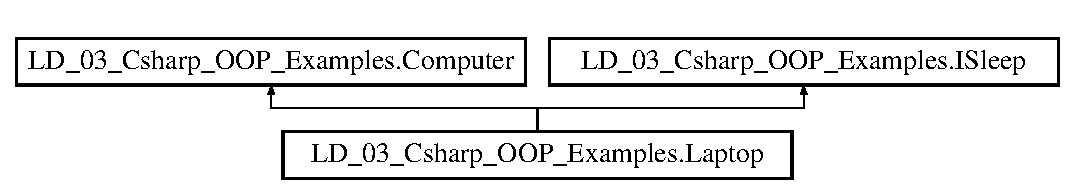
\includegraphics[height=2.000000cm]{class_l_d__03___csharp___o_o_p___examples_1_1_laptop}
\end{center}
\end{figure}
\subsection*{Public Member Functions}
\begin{DoxyCompactItemize}
\item 
\mbox{\hyperlink{class_l_d__03___csharp___o_o_p___examples_1_1_laptop_a8221274b4d3b4d05eff718d010e0eefa}{Laptop}} (string name, int width, int heigth)
\item 
void \mbox{\hyperlink{class_l_d__03___csharp___o_o_p___examples_1_1_laptop_a28f09dd23331929b11cdc77720153e21}{Toggle\+Sleep}} ()
\end{DoxyCompactItemize}
\subsection*{Public Attributes}
\begin{DoxyCompactItemize}
\item 
\mbox{\hyperlink{interface_l_d__03___csharp___o_o_p___examples_1_1_i_sleep}{I\+Sleep}} \mbox{\hyperlink{class_l_d__03___csharp___o_o_p___examples_1_1_laptop_aabaead761ad3ae86e24f66e24d26fe31}{sleep\+Controller}}
\end{DoxyCompactItemize}
\subsection*{Properties}
\begin{DoxyCompactItemize}
\item 
\mbox{\hyperlink{class_l_d__03___csharp___o_o_p___examples_1_1_display}{Display}} \mbox{\hyperlink{class_l_d__03___csharp___o_o_p___examples_1_1_laptop_a38fa411e5013b052b67d7e2e4a32c816}{Display}}\hspace{0.3cm}{\ttfamily  \mbox{[}get\mbox{]}}
\item 
bool \mbox{\hyperlink{class_l_d__03___csharp___o_o_p___examples_1_1_laptop_aaefe6924fee73daa583243aaea602a13}{Is\+Sleeping}}\hspace{0.3cm}{\ttfamily  \mbox{[}get\mbox{]}}
\end{DoxyCompactItemize}
\subsection*{Additional Inherited Members}


\subsection{Constructor \& Destructor Documentation}
\mbox{\Hypertarget{class_l_d__03___csharp___o_o_p___examples_1_1_laptop_a8221274b4d3b4d05eff718d010e0eefa}\label{class_l_d__03___csharp___o_o_p___examples_1_1_laptop_a8221274b4d3b4d05eff718d010e0eefa}} 
\index{L\+D\+\_\+03\+\_\+\+Csharp\+\_\+\+O\+O\+P\+\_\+\+Examples\+::\+Laptop@{L\+D\+\_\+03\+\_\+\+Csharp\+\_\+\+O\+O\+P\+\_\+\+Examples\+::\+Laptop}!Laptop@{Laptop}}
\index{Laptop@{Laptop}!L\+D\+\_\+03\+\_\+\+Csharp\+\_\+\+O\+O\+P\+\_\+\+Examples\+::\+Laptop@{L\+D\+\_\+03\+\_\+\+Csharp\+\_\+\+O\+O\+P\+\_\+\+Examples\+::\+Laptop}}
\subsubsection{\texorpdfstring{Laptop()}{Laptop()}}
{\footnotesize\ttfamily L\+D\+\_\+03\+\_\+\+Csharp\+\_\+\+O\+O\+P\+\_\+\+Examples.\+Laptop.\+Laptop (\begin{DoxyParamCaption}\item[{string}]{name,  }\item[{int}]{width,  }\item[{int}]{heigth }\end{DoxyParamCaption})}



\subsection{Member Function Documentation}
\mbox{\Hypertarget{class_l_d__03___csharp___o_o_p___examples_1_1_laptop_a28f09dd23331929b11cdc77720153e21}\label{class_l_d__03___csharp___o_o_p___examples_1_1_laptop_a28f09dd23331929b11cdc77720153e21}} 
\index{L\+D\+\_\+03\+\_\+\+Csharp\+\_\+\+O\+O\+P\+\_\+\+Examples\+::\+Laptop@{L\+D\+\_\+03\+\_\+\+Csharp\+\_\+\+O\+O\+P\+\_\+\+Examples\+::\+Laptop}!Toggle\+Sleep@{Toggle\+Sleep}}
\index{Toggle\+Sleep@{Toggle\+Sleep}!L\+D\+\_\+03\+\_\+\+Csharp\+\_\+\+O\+O\+P\+\_\+\+Examples\+::\+Laptop@{L\+D\+\_\+03\+\_\+\+Csharp\+\_\+\+O\+O\+P\+\_\+\+Examples\+::\+Laptop}}
\subsubsection{\texorpdfstring{Toggle\+Sleep()}{ToggleSleep()}}
{\footnotesize\ttfamily void L\+D\+\_\+03\+\_\+\+Csharp\+\_\+\+O\+O\+P\+\_\+\+Examples.\+Laptop.\+Toggle\+Sleep (\begin{DoxyParamCaption}{ }\end{DoxyParamCaption})}



Implements \mbox{\hyperlink{interface_l_d__03___csharp___o_o_p___examples_1_1_i_sleep_a51a16beac9cf61fd4d088e169790bd08}{L\+D\+\_\+03\+\_\+\+Csharp\+\_\+\+O\+O\+P\+\_\+\+Examples.\+I\+Sleep}}.



\subsection{Member Data Documentation}
\mbox{\Hypertarget{class_l_d__03___csharp___o_o_p___examples_1_1_laptop_aabaead761ad3ae86e24f66e24d26fe31}\label{class_l_d__03___csharp___o_o_p___examples_1_1_laptop_aabaead761ad3ae86e24f66e24d26fe31}} 
\index{L\+D\+\_\+03\+\_\+\+Csharp\+\_\+\+O\+O\+P\+\_\+\+Examples\+::\+Laptop@{L\+D\+\_\+03\+\_\+\+Csharp\+\_\+\+O\+O\+P\+\_\+\+Examples\+::\+Laptop}!sleep\+Controller@{sleep\+Controller}}
\index{sleep\+Controller@{sleep\+Controller}!L\+D\+\_\+03\+\_\+\+Csharp\+\_\+\+O\+O\+P\+\_\+\+Examples\+::\+Laptop@{L\+D\+\_\+03\+\_\+\+Csharp\+\_\+\+O\+O\+P\+\_\+\+Examples\+::\+Laptop}}
\subsubsection{\texorpdfstring{sleep\+Controller}{sleepController}}
{\footnotesize\ttfamily \mbox{\hyperlink{interface_l_d__03___csharp___o_o_p___examples_1_1_i_sleep}{I\+Sleep}} L\+D\+\_\+03\+\_\+\+Csharp\+\_\+\+O\+O\+P\+\_\+\+Examples.\+Laptop.\+sleep\+Controller}



\subsection{Property Documentation}
\mbox{\Hypertarget{class_l_d__03___csharp___o_o_p___examples_1_1_laptop_a38fa411e5013b052b67d7e2e4a32c816}\label{class_l_d__03___csharp___o_o_p___examples_1_1_laptop_a38fa411e5013b052b67d7e2e4a32c816}} 
\index{L\+D\+\_\+03\+\_\+\+Csharp\+\_\+\+O\+O\+P\+\_\+\+Examples\+::\+Laptop@{L\+D\+\_\+03\+\_\+\+Csharp\+\_\+\+O\+O\+P\+\_\+\+Examples\+::\+Laptop}!Display@{Display}}
\index{Display@{Display}!L\+D\+\_\+03\+\_\+\+Csharp\+\_\+\+O\+O\+P\+\_\+\+Examples\+::\+Laptop@{L\+D\+\_\+03\+\_\+\+Csharp\+\_\+\+O\+O\+P\+\_\+\+Examples\+::\+Laptop}}
\subsubsection{\texorpdfstring{Display}{Display}}
{\footnotesize\ttfamily \mbox{\hyperlink{class_l_d__03___csharp___o_o_p___examples_1_1_display}{Display}} L\+D\+\_\+03\+\_\+\+Csharp\+\_\+\+O\+O\+P\+\_\+\+Examples.\+Laptop.\+Display\hspace{0.3cm}{\ttfamily [get]}}

\mbox{\Hypertarget{class_l_d__03___csharp___o_o_p___examples_1_1_laptop_aaefe6924fee73daa583243aaea602a13}\label{class_l_d__03___csharp___o_o_p___examples_1_1_laptop_aaefe6924fee73daa583243aaea602a13}} 
\index{L\+D\+\_\+03\+\_\+\+Csharp\+\_\+\+O\+O\+P\+\_\+\+Examples\+::\+Laptop@{L\+D\+\_\+03\+\_\+\+Csharp\+\_\+\+O\+O\+P\+\_\+\+Examples\+::\+Laptop}!Is\+Sleeping@{Is\+Sleeping}}
\index{Is\+Sleeping@{Is\+Sleeping}!L\+D\+\_\+03\+\_\+\+Csharp\+\_\+\+O\+O\+P\+\_\+\+Examples\+::\+Laptop@{L\+D\+\_\+03\+\_\+\+Csharp\+\_\+\+O\+O\+P\+\_\+\+Examples\+::\+Laptop}}
\subsubsection{\texorpdfstring{Is\+Sleeping}{IsSleeping}}
{\footnotesize\ttfamily bool L\+D\+\_\+03\+\_\+\+Csharp\+\_\+\+O\+O\+P\+\_\+\+Examples.\+Laptop.\+Is\+Sleeping\hspace{0.3cm}{\ttfamily [get]}}



The documentation for this class was generated from the following file\+:\begin{DoxyCompactItemize}
\item 
C\+:/\+Users/thead/source/repos/\+L\+D-\/03-\/\+Csharp-\/\+O\+O\+P-\/\+Examples/\mbox{\hyperlink{_laptop_8cs}{Laptop.\+cs}}\end{DoxyCompactItemize}

\hypertarget{class_l_d__03___csharp___o_o_p___examples_1_1_power_controller}{}\section{L\+D\+\_\+03\+\_\+\+Csharp\+\_\+\+O\+O\+P\+\_\+\+Examples.\+Power\+Controller Class Reference}
\label{class_l_d__03___csharp___o_o_p___examples_1_1_power_controller}\index{L\+D\+\_\+03\+\_\+\+Csharp\+\_\+\+O\+O\+P\+\_\+\+Examples.\+Power\+Controller@{L\+D\+\_\+03\+\_\+\+Csharp\+\_\+\+O\+O\+P\+\_\+\+Examples.\+Power\+Controller}}
Inheritance diagram for L\+D\+\_\+03\+\_\+\+Csharp\+\_\+\+O\+O\+P\+\_\+\+Examples.\+Power\+Controller\+:\begin{figure}[H]
\begin{center}
\leavevmode
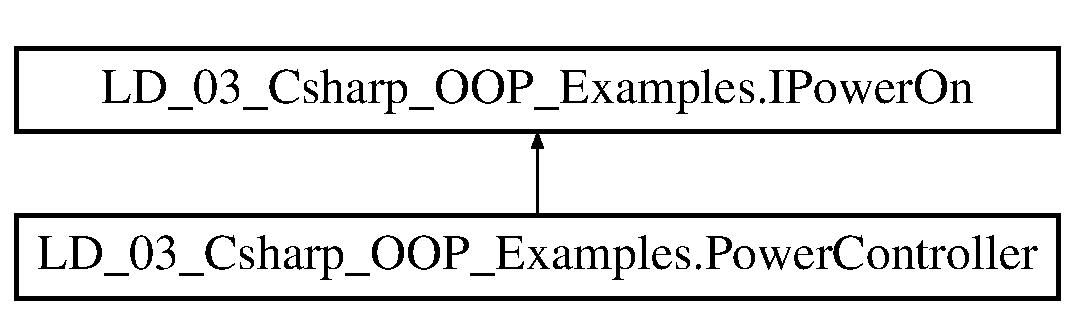
\includegraphics[height=2.000000cm]{class_l_d__03___csharp___o_o_p___examples_1_1_power_controller}
\end{center}
\end{figure}
\subsection*{Public Member Functions}
\begin{DoxyCompactItemize}
\item 
virtual void \mbox{\hyperlink{class_l_d__03___csharp___o_o_p___examples_1_1_power_controller_accb660a5257db2d4d1df4e35d4147027}{Toggle\+Power}} ()
\end{DoxyCompactItemize}
\subsection*{Protected Member Functions}
\begin{DoxyCompactItemize}
\item 
void \mbox{\hyperlink{class_l_d__03___csharp___o_o_p___examples_1_1_power_controller_aac6ffd8e2256a46a26b344cd2846ed90}{Turn\+On}} ()
\item 
void \mbox{\hyperlink{class_l_d__03___csharp___o_o_p___examples_1_1_power_controller_a60438bf1fbf976ad624eb18f8d8d7edb}{Turn\+Off}} ()
\end{DoxyCompactItemize}
\subsection*{Properties}
\begin{DoxyCompactItemize}
\item 
bool \mbox{\hyperlink{class_l_d__03___csharp___o_o_p___examples_1_1_power_controller_a1e3e0b435604ac040029c0c3df851a97}{Is\+On}}\hspace{0.3cm}{\ttfamily  \mbox{[}get\mbox{]}}
\end{DoxyCompactItemize}


\subsection{Member Function Documentation}
\mbox{\Hypertarget{class_l_d__03___csharp___o_o_p___examples_1_1_power_controller_accb660a5257db2d4d1df4e35d4147027}\label{class_l_d__03___csharp___o_o_p___examples_1_1_power_controller_accb660a5257db2d4d1df4e35d4147027}} 
\index{L\+D\+\_\+03\+\_\+\+Csharp\+\_\+\+O\+O\+P\+\_\+\+Examples\+::\+Power\+Controller@{L\+D\+\_\+03\+\_\+\+Csharp\+\_\+\+O\+O\+P\+\_\+\+Examples\+::\+Power\+Controller}!Toggle\+Power@{Toggle\+Power}}
\index{Toggle\+Power@{Toggle\+Power}!L\+D\+\_\+03\+\_\+\+Csharp\+\_\+\+O\+O\+P\+\_\+\+Examples\+::\+Power\+Controller@{L\+D\+\_\+03\+\_\+\+Csharp\+\_\+\+O\+O\+P\+\_\+\+Examples\+::\+Power\+Controller}}
\subsubsection{\texorpdfstring{Toggle\+Power()}{TogglePower()}}
{\footnotesize\ttfamily virtual void L\+D\+\_\+03\+\_\+\+Csharp\+\_\+\+O\+O\+P\+\_\+\+Examples.\+Power\+Controller.\+Toggle\+Power (\begin{DoxyParamCaption}{ }\end{DoxyParamCaption})\hspace{0.3cm}{\ttfamily [virtual]}}



Implements \mbox{\hyperlink{interface_l_d__03___csharp___o_o_p___examples_1_1_i_power_on_a6f71e842b3e94a5d6d690671197d0adc}{L\+D\+\_\+03\+\_\+\+Csharp\+\_\+\+O\+O\+P\+\_\+\+Examples.\+I\+Power\+On}}.

\mbox{\Hypertarget{class_l_d__03___csharp___o_o_p___examples_1_1_power_controller_a60438bf1fbf976ad624eb18f8d8d7edb}\label{class_l_d__03___csharp___o_o_p___examples_1_1_power_controller_a60438bf1fbf976ad624eb18f8d8d7edb}} 
\index{L\+D\+\_\+03\+\_\+\+Csharp\+\_\+\+O\+O\+P\+\_\+\+Examples\+::\+Power\+Controller@{L\+D\+\_\+03\+\_\+\+Csharp\+\_\+\+O\+O\+P\+\_\+\+Examples\+::\+Power\+Controller}!Turn\+Off@{Turn\+Off}}
\index{Turn\+Off@{Turn\+Off}!L\+D\+\_\+03\+\_\+\+Csharp\+\_\+\+O\+O\+P\+\_\+\+Examples\+::\+Power\+Controller@{L\+D\+\_\+03\+\_\+\+Csharp\+\_\+\+O\+O\+P\+\_\+\+Examples\+::\+Power\+Controller}}
\subsubsection{\texorpdfstring{Turn\+Off()}{TurnOff()}}
{\footnotesize\ttfamily void L\+D\+\_\+03\+\_\+\+Csharp\+\_\+\+O\+O\+P\+\_\+\+Examples.\+Power\+Controller.\+Turn\+Off (\begin{DoxyParamCaption}{ }\end{DoxyParamCaption})\hspace{0.3cm}{\ttfamily [protected]}}

\mbox{\Hypertarget{class_l_d__03___csharp___o_o_p___examples_1_1_power_controller_aac6ffd8e2256a46a26b344cd2846ed90}\label{class_l_d__03___csharp___o_o_p___examples_1_1_power_controller_aac6ffd8e2256a46a26b344cd2846ed90}} 
\index{L\+D\+\_\+03\+\_\+\+Csharp\+\_\+\+O\+O\+P\+\_\+\+Examples\+::\+Power\+Controller@{L\+D\+\_\+03\+\_\+\+Csharp\+\_\+\+O\+O\+P\+\_\+\+Examples\+::\+Power\+Controller}!Turn\+On@{Turn\+On}}
\index{Turn\+On@{Turn\+On}!L\+D\+\_\+03\+\_\+\+Csharp\+\_\+\+O\+O\+P\+\_\+\+Examples\+::\+Power\+Controller@{L\+D\+\_\+03\+\_\+\+Csharp\+\_\+\+O\+O\+P\+\_\+\+Examples\+::\+Power\+Controller}}
\subsubsection{\texorpdfstring{Turn\+On()}{TurnOn()}}
{\footnotesize\ttfamily void L\+D\+\_\+03\+\_\+\+Csharp\+\_\+\+O\+O\+P\+\_\+\+Examples.\+Power\+Controller.\+Turn\+On (\begin{DoxyParamCaption}{ }\end{DoxyParamCaption})\hspace{0.3cm}{\ttfamily [protected]}}



\subsection{Property Documentation}
\mbox{\Hypertarget{class_l_d__03___csharp___o_o_p___examples_1_1_power_controller_a1e3e0b435604ac040029c0c3df851a97}\label{class_l_d__03___csharp___o_o_p___examples_1_1_power_controller_a1e3e0b435604ac040029c0c3df851a97}} 
\index{L\+D\+\_\+03\+\_\+\+Csharp\+\_\+\+O\+O\+P\+\_\+\+Examples\+::\+Power\+Controller@{L\+D\+\_\+03\+\_\+\+Csharp\+\_\+\+O\+O\+P\+\_\+\+Examples\+::\+Power\+Controller}!Is\+On@{Is\+On}}
\index{Is\+On@{Is\+On}!L\+D\+\_\+03\+\_\+\+Csharp\+\_\+\+O\+O\+P\+\_\+\+Examples\+::\+Power\+Controller@{L\+D\+\_\+03\+\_\+\+Csharp\+\_\+\+O\+O\+P\+\_\+\+Examples\+::\+Power\+Controller}}
\subsubsection{\texorpdfstring{Is\+On}{IsOn}}
{\footnotesize\ttfamily bool L\+D\+\_\+03\+\_\+\+Csharp\+\_\+\+O\+O\+P\+\_\+\+Examples.\+Power\+Controller.\+Is\+On\hspace{0.3cm}{\ttfamily [get]}}



The documentation for this class was generated from the following file\+:\begin{DoxyCompactItemize}
\item 
C\+:/\+Users/thead/source/repos/\+L\+D-\/03-\/\+Csharp-\/\+O\+O\+P-\/\+Examples/\mbox{\hyperlink{_power_controller_8cs}{Power\+Controller.\+cs}}\end{DoxyCompactItemize}

\hypertarget{class_program}{}\section{Program Class Reference}
\label{class_program}\index{Program@{Program}}


The documentation for this class was generated from the following file\+:\begin{DoxyCompactItemize}
\item 
C\+:/\+Users/thead/source/repos/\+L\+D-\/03-\/\+Csharp-\/\+O\+O\+P-\/\+Examples/\mbox{\hyperlink{_program_8cs}{Program.\+cs}}\end{DoxyCompactItemize}

\hypertarget{class_l_d__03___csharp___o_o_p___examples_1_1_sleep_controler}{}\section{L\+D\+\_\+03\+\_\+\+Csharp\+\_\+\+O\+O\+P\+\_\+\+Examples.\+Sleep\+Controler Class Reference}
\label{class_l_d__03___csharp___o_o_p___examples_1_1_sleep_controler}\index{L\+D\+\_\+03\+\_\+\+Csharp\+\_\+\+O\+O\+P\+\_\+\+Examples.\+Sleep\+Controler@{L\+D\+\_\+03\+\_\+\+Csharp\+\_\+\+O\+O\+P\+\_\+\+Examples.\+Sleep\+Controler}}
Inheritance diagram for L\+D\+\_\+03\+\_\+\+Csharp\+\_\+\+O\+O\+P\+\_\+\+Examples.\+Sleep\+Controler\+:\begin{figure}[H]
\begin{center}
\leavevmode
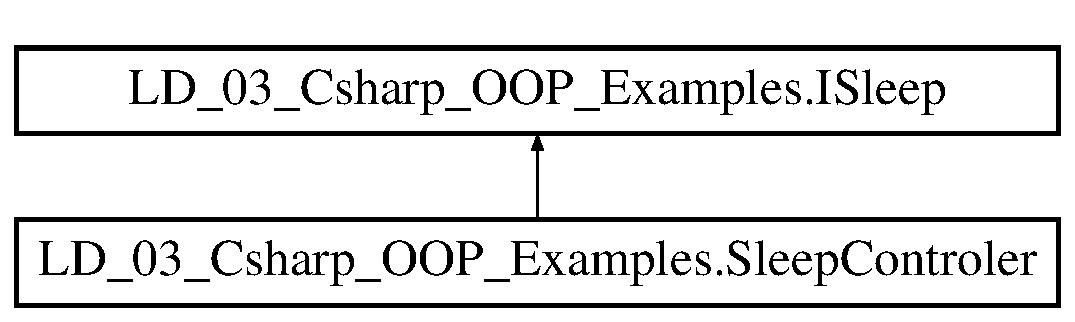
\includegraphics[height=2.000000cm]{class_l_d__03___csharp___o_o_p___examples_1_1_sleep_controler}
\end{center}
\end{figure}
\subsection*{Public Member Functions}
\begin{DoxyCompactItemize}
\item 
void \mbox{\hyperlink{class_l_d__03___csharp___o_o_p___examples_1_1_sleep_controler_ad8b90b3fa29e24828b2d739961458dba}{Toggle\+Sleep}} ()
\end{DoxyCompactItemize}
\subsection*{Properties}
\begin{DoxyCompactItemize}
\item 
bool \mbox{\hyperlink{class_l_d__03___csharp___o_o_p___examples_1_1_sleep_controler_ae68167d3360f4f9b0a7bec48ab64e898}{Is\+Sleeping}}\hspace{0.3cm}{\ttfamily  \mbox{[}get\mbox{]}}
\end{DoxyCompactItemize}


\subsection{Member Function Documentation}
\mbox{\Hypertarget{class_l_d__03___csharp___o_o_p___examples_1_1_sleep_controler_ad8b90b3fa29e24828b2d739961458dba}\label{class_l_d__03___csharp___o_o_p___examples_1_1_sleep_controler_ad8b90b3fa29e24828b2d739961458dba}} 
\index{L\+D\+\_\+03\+\_\+\+Csharp\+\_\+\+O\+O\+P\+\_\+\+Examples\+::\+Sleep\+Controler@{L\+D\+\_\+03\+\_\+\+Csharp\+\_\+\+O\+O\+P\+\_\+\+Examples\+::\+Sleep\+Controler}!Toggle\+Sleep@{Toggle\+Sleep}}
\index{Toggle\+Sleep@{Toggle\+Sleep}!L\+D\+\_\+03\+\_\+\+Csharp\+\_\+\+O\+O\+P\+\_\+\+Examples\+::\+Sleep\+Controler@{L\+D\+\_\+03\+\_\+\+Csharp\+\_\+\+O\+O\+P\+\_\+\+Examples\+::\+Sleep\+Controler}}
\subsubsection{\texorpdfstring{Toggle\+Sleep()}{ToggleSleep()}}
{\footnotesize\ttfamily void L\+D\+\_\+03\+\_\+\+Csharp\+\_\+\+O\+O\+P\+\_\+\+Examples.\+Sleep\+Controler.\+Toggle\+Sleep (\begin{DoxyParamCaption}{ }\end{DoxyParamCaption})}



Implements \mbox{\hyperlink{interface_l_d__03___csharp___o_o_p___examples_1_1_i_sleep_a51a16beac9cf61fd4d088e169790bd08}{L\+D\+\_\+03\+\_\+\+Csharp\+\_\+\+O\+O\+P\+\_\+\+Examples.\+I\+Sleep}}.



\subsection{Property Documentation}
\mbox{\Hypertarget{class_l_d__03___csharp___o_o_p___examples_1_1_sleep_controler_ae68167d3360f4f9b0a7bec48ab64e898}\label{class_l_d__03___csharp___o_o_p___examples_1_1_sleep_controler_ae68167d3360f4f9b0a7bec48ab64e898}} 
\index{L\+D\+\_\+03\+\_\+\+Csharp\+\_\+\+O\+O\+P\+\_\+\+Examples\+::\+Sleep\+Controler@{L\+D\+\_\+03\+\_\+\+Csharp\+\_\+\+O\+O\+P\+\_\+\+Examples\+::\+Sleep\+Controler}!Is\+Sleeping@{Is\+Sleeping}}
\index{Is\+Sleeping@{Is\+Sleeping}!L\+D\+\_\+03\+\_\+\+Csharp\+\_\+\+O\+O\+P\+\_\+\+Examples\+::\+Sleep\+Controler@{L\+D\+\_\+03\+\_\+\+Csharp\+\_\+\+O\+O\+P\+\_\+\+Examples\+::\+Sleep\+Controler}}
\subsubsection{\texorpdfstring{Is\+Sleeping}{IsSleeping}}
{\footnotesize\ttfamily bool L\+D\+\_\+03\+\_\+\+Csharp\+\_\+\+O\+O\+P\+\_\+\+Examples.\+Sleep\+Controler.\+Is\+Sleeping\hspace{0.3cm}{\ttfamily [get]}}



The documentation for this class was generated from the following file\+:\begin{DoxyCompactItemize}
\item 
C\+:/\+Users/thead/source/repos/\+L\+D-\/03-\/\+Csharp-\/\+O\+O\+P-\/\+Examples/\mbox{\hyperlink{_sleep_controler_8cs}{Sleep\+Controler.\+cs}}\end{DoxyCompactItemize}

\chapter{File Documentation}
\hypertarget{_computer_8cs}{}\section{C\+:/\+Users/thead/source/repos/\+L\+D-\/03-\/\+Csharp-\/\+O\+O\+P-\/\+Examples/\+Computer.cs File Reference}
\label{_computer_8cs}\index{C\+:/\+Users/thead/source/repos/\+L\+D-\/03-\/\+Csharp-\/\+O\+O\+P-\/\+Examples/\+Computer.\+cs@{C\+:/\+Users/thead/source/repos/\+L\+D-\/03-\/\+Csharp-\/\+O\+O\+P-\/\+Examples/\+Computer.\+cs}}
\subsection*{Classes}
\begin{DoxyCompactItemize}
\item 
class \mbox{\hyperlink{class_l_d__03___csharp___o_o_p___examples_1_1_computer}{L\+D\+\_\+03\+\_\+\+Csharp\+\_\+\+O\+O\+P\+\_\+\+Examples.\+Computer}}
\end{DoxyCompactItemize}
\subsection*{Namespaces}
\begin{DoxyCompactItemize}
\item 
namespace \mbox{\hyperlink{namespace_l_d__03___csharp___o_o_p___examples}{L\+D\+\_\+03\+\_\+\+Csharp\+\_\+\+O\+O\+P\+\_\+\+Examples}}
\end{DoxyCompactItemize}

\hypertarget{_desktop_8cs}{}\section{C\+:/\+Users/thead/source/repos/\+L\+D-\/03-\/\+Csharp-\/\+O\+O\+P-\/\+Examples/\+Desktop.cs File Reference}
\label{_desktop_8cs}\index{C\+:/\+Users/thead/source/repos/\+L\+D-\/03-\/\+Csharp-\/\+O\+O\+P-\/\+Examples/\+Desktop.\+cs@{C\+:/\+Users/thead/source/repos/\+L\+D-\/03-\/\+Csharp-\/\+O\+O\+P-\/\+Examples/\+Desktop.\+cs}}
\subsection*{Classes}
\begin{DoxyCompactItemize}
\item 
class \mbox{\hyperlink{class_o_o_p_examples_1_1_computer}{O\+O\+P\+Examples.\+Computer}}
\end{DoxyCompactItemize}
\subsection*{Namespaces}
\begin{DoxyCompactItemize}
\item 
namespace \mbox{\hyperlink{namespace_o_o_p_examples}{O\+O\+P\+Examples}}
\end{DoxyCompactItemize}

\hypertarget{_display_8cs}{}\section{C\+:/\+Users/thead/source/repos/\+L\+D-\/03-\/\+Csharp-\/\+O\+O\+P-\/\+Examples/\+Display.cs File Reference}
\label{_display_8cs}\index{C\+:/\+Users/thead/source/repos/\+L\+D-\/03-\/\+Csharp-\/\+O\+O\+P-\/\+Examples/\+Display.\+cs@{C\+:/\+Users/thead/source/repos/\+L\+D-\/03-\/\+Csharp-\/\+O\+O\+P-\/\+Examples/\+Display.\+cs}}
\subsection*{Classes}
\begin{DoxyCompactItemize}
\item 
class \mbox{\hyperlink{class_l_d__03___csharp___o_o_p___examples_1_1_display}{L\+D\+\_\+03\+\_\+\+Csharp\+\_\+\+O\+O\+P\+\_\+\+Examples.\+Display}}
\end{DoxyCompactItemize}
\subsection*{Namespaces}
\begin{DoxyCompactItemize}
\item 
namespace \mbox{\hyperlink{namespace_l_d__03___csharp___o_o_p___examples}{L\+D\+\_\+03\+\_\+\+Csharp\+\_\+\+O\+O\+P\+\_\+\+Examples}}
\end{DoxyCompactItemize}

\hypertarget{_i_power_on_8cs}{}\section{C\+:/\+Users/thead/source/repos/\+L\+D-\/03-\/\+Csharp-\/\+O\+O\+P-\/\+Examples/\+I\+Power\+On.cs File Reference}
\label{_i_power_on_8cs}\index{C\+:/\+Users/thead/source/repos/\+L\+D-\/03-\/\+Csharp-\/\+O\+O\+P-\/\+Examples/\+I\+Power\+On.\+cs@{C\+:/\+Users/thead/source/repos/\+L\+D-\/03-\/\+Csharp-\/\+O\+O\+P-\/\+Examples/\+I\+Power\+On.\+cs}}
\subsection*{Classes}
\begin{DoxyCompactItemize}
\item 
interface \mbox{\hyperlink{interface_l_d__03___csharp___o_o_p___examples_1_1_i_power_on}{L\+D\+\_\+03\+\_\+\+Csharp\+\_\+\+O\+O\+P\+\_\+\+Examples.\+I\+Power\+On}}
\end{DoxyCompactItemize}
\subsection*{Namespaces}
\begin{DoxyCompactItemize}
\item 
namespace \mbox{\hyperlink{namespace_l_d__03___csharp___o_o_p___examples}{L\+D\+\_\+03\+\_\+\+Csharp\+\_\+\+O\+O\+P\+\_\+\+Examples}}
\end{DoxyCompactItemize}

\hypertarget{_i_sleep_8cs}{}\section{C\+:/\+Users/thead/source/repos/\+L\+D-\/03-\/\+Csharp-\/\+O\+O\+P-\/\+Examples/\+I\+Sleep.cs File Reference}
\label{_i_sleep_8cs}\index{C\+:/\+Users/thead/source/repos/\+L\+D-\/03-\/\+Csharp-\/\+O\+O\+P-\/\+Examples/\+I\+Sleep.\+cs@{C\+:/\+Users/thead/source/repos/\+L\+D-\/03-\/\+Csharp-\/\+O\+O\+P-\/\+Examples/\+I\+Sleep.\+cs}}
\subsection*{Classes}
\begin{DoxyCompactItemize}
\item 
interface \mbox{\hyperlink{interface_l_d__03___csharp___o_o_p___examples_1_1_i_sleep}{L\+D\+\_\+03\+\_\+\+Csharp\+\_\+\+O\+O\+P\+\_\+\+Examples.\+I\+Sleep}}
\end{DoxyCompactItemize}
\subsection*{Namespaces}
\begin{DoxyCompactItemize}
\item 
namespace \mbox{\hyperlink{namespace_l_d__03___csharp___o_o_p___examples}{L\+D\+\_\+03\+\_\+\+Csharp\+\_\+\+O\+O\+P\+\_\+\+Examples}}
\end{DoxyCompactItemize}

\hypertarget{_laptop_8cs}{}\section{C\+:/\+Users/thead/source/repos/\+L\+D-\/03-\/\+Csharp-\/\+O\+O\+P-\/\+Examples/\+Laptop.cs File Reference}
\label{_laptop_8cs}\index{C\+:/\+Users/thead/source/repos/\+L\+D-\/03-\/\+Csharp-\/\+O\+O\+P-\/\+Examples/\+Laptop.\+cs@{C\+:/\+Users/thead/source/repos/\+L\+D-\/03-\/\+Csharp-\/\+O\+O\+P-\/\+Examples/\+Laptop.\+cs}}
\subsection*{Classes}
\begin{DoxyCompactItemize}
\item 
class \mbox{\hyperlink{class_l_d__03___csharp___o_o_p___examples_1_1_laptop}{L\+D\+\_\+03\+\_\+\+Csharp\+\_\+\+O\+O\+P\+\_\+\+Examples.\+Laptop}}
\end{DoxyCompactItemize}
\subsection*{Namespaces}
\begin{DoxyCompactItemize}
\item 
namespace \mbox{\hyperlink{namespace_l_d__03___csharp___o_o_p___examples}{L\+D\+\_\+03\+\_\+\+Csharp\+\_\+\+O\+O\+P\+\_\+\+Examples}}
\end{DoxyCompactItemize}

\hypertarget{_power_controller_8cs}{}\section{C\+:/\+Users/thead/source/repos/\+L\+D-\/03-\/\+Csharp-\/\+O\+O\+P-\/\+Examples/\+Power\+Controller.cs File Reference}
\label{_power_controller_8cs}\index{C\+:/\+Users/thead/source/repos/\+L\+D-\/03-\/\+Csharp-\/\+O\+O\+P-\/\+Examples/\+Power\+Controller.\+cs@{C\+:/\+Users/thead/source/repos/\+L\+D-\/03-\/\+Csharp-\/\+O\+O\+P-\/\+Examples/\+Power\+Controller.\+cs}}
\subsection*{Classes}
\begin{DoxyCompactItemize}
\item 
class \mbox{\hyperlink{class_l_d__03___csharp___o_o_p___examples_1_1_power_controller}{L\+D\+\_\+03\+\_\+\+Csharp\+\_\+\+O\+O\+P\+\_\+\+Examples.\+Power\+Controller}}
\end{DoxyCompactItemize}
\subsection*{Namespaces}
\begin{DoxyCompactItemize}
\item 
namespace \mbox{\hyperlink{namespace_l_d__03___csharp___o_o_p___examples}{L\+D\+\_\+03\+\_\+\+Csharp\+\_\+\+O\+O\+P\+\_\+\+Examples}}
\end{DoxyCompactItemize}

\hypertarget{_program_8cs}{}\section{C\+:/\+Users/thead/source/repos/\+L\+D-\/03-\/\+Csharp-\/\+O\+O\+P-\/\+Examples/\+Program.cs File Reference}
\label{_program_8cs}\index{C\+:/\+Users/thead/source/repos/\+L\+D-\/03-\/\+Csharp-\/\+O\+O\+P-\/\+Examples/\+Program.\+cs@{C\+:/\+Users/thead/source/repos/\+L\+D-\/03-\/\+Csharp-\/\+O\+O\+P-\/\+Examples/\+Program.\+cs}}
\subsection*{Classes}
\begin{DoxyCompactItemize}
\item 
class \mbox{\hyperlink{class_program}{Program}}
\end{DoxyCompactItemize}

\hypertarget{_sleep_controler_8cs}{}\section{C\+:/\+Users/thead/source/repos/\+L\+D-\/03-\/\+Csharp-\/\+O\+O\+P-\/\+Examples/\+Sleep\+Controler.cs File Reference}
\label{_sleep_controler_8cs}\index{C\+:/\+Users/thead/source/repos/\+L\+D-\/03-\/\+Csharp-\/\+O\+O\+P-\/\+Examples/\+Sleep\+Controler.\+cs@{C\+:/\+Users/thead/source/repos/\+L\+D-\/03-\/\+Csharp-\/\+O\+O\+P-\/\+Examples/\+Sleep\+Controler.\+cs}}
\subsection*{Classes}
\begin{DoxyCompactItemize}
\item 
class \mbox{\hyperlink{class_l_d__03___csharp___o_o_p___examples_1_1_sleep_controler}{L\+D\+\_\+03\+\_\+\+Csharp\+\_\+\+O\+O\+P\+\_\+\+Examples.\+Sleep\+Controler}}
\end{DoxyCompactItemize}
\subsection*{Namespaces}
\begin{DoxyCompactItemize}
\item 
namespace \mbox{\hyperlink{namespace_l_d__03___csharp___o_o_p___examples}{L\+D\+\_\+03\+\_\+\+Csharp\+\_\+\+O\+O\+P\+\_\+\+Examples}}
\end{DoxyCompactItemize}

%--- End generated contents ---

% Index
\backmatter
\newpage
\phantomsection
\clearemptydoublepage
\addcontentsline{toc}{chapter}{Index}
\printindex

\end{document}
